\chapter{Schüler UI, Anbindung an die Schnittstelle und Entwicklung des Mathe Piano Spiels}
Christian Pfeiffer, Normen Krug \& \href{mailto:jofranz90@gmail.com?subject=Swift-Studienarbeit}{Johannes Franz}


\section{Einleitung}
In diesem Abschnitt werden die Ziele und die Motivation des Projektes definiert. Dabei werden unter anderem die Erwartungen an das Projekt genannt.

\subsection{Motivation}
Die Hauptmotivation des Projektes war das Lernen und Einarbeiten in neue Apple Frameworks (wie \textit{SpriteKit} und \textit{CloudKit}) und Erfahrungen sammeln in der Zusammenarbeit mit mehreren Entwicklerteams, welche gleichzeitig an einem Projekt arbeiten. Deshalb war es zwingend notwendig, sich mit anderen Teams zu verständigen und auszutauschen.  

\subsection{Ziele}
Als Ziele der Studienarbeit wurden folgende Punkte definiert: 
\begin{itemize}
\item Kinderfreundliches Design und Layout
\item Erstellen eines Mathelernspieles 
\item Aufgaben die von Lehrern erstellt werden anzeigen und in ein spielbare Form überführen
\item Die von Schüler beantworteten Fragen an den Lehrer weiterleiten
\item Den Schülern die Möglichkeit bieten die Spiele im Endlos Modus, unabhängig der von Lehrer zugewiesenen Aufgaben, zu spielen
\item Lernen eines neuen Apple Frameworks (\textit{SpriteKit})
\item Erfahrung sammeln in Zusammenarbeit mit anderen Teams
\end{itemize}
\section{Spezifikation}
Als Strategie für die Umsetzung des Projektes wurde das Prinzip "Funktionalität vor UI-Design" gewählt. Als die Funktionalität dann zufriedenstellend.

\subsection{Mathe Piano Spiel}
Bei der Entwicklung des Spiels war es wichtig, möglichst schnell einen funktionsfähigen Prototypen zu ertstellen. Dieser wurde im Verlauf des Projektes immer weiter verbessert.


\subsubsection{Game Engine}
Als Grundlage wurde die von Apple entwickelte Game Engine namens \textit{SpriteKit} verwenden. Diese Engine hat einige Vorteile gegenüber anderen Spielengines:
\begin{itemize}
\item Gute Dokumentation
\item Wiederverwendungen bereits gelernter Paradigmen    
\item Einfache Integrationsmöglichkeit in die App
\item Einfache Anbindung an andere iOS API‘s
\item Swift als Programmiersprache 
\item Schnelles Entwickeln und Testen von Funktionen durch Swift Playgrounds
\end{itemize}

\subsubsection{Herausforderungen}
Nach der ausgiebigen Einarbeitung in das \textit{SpriteKit} \textit{Framework} haben sich einige Hürden ergeben. Das Verwenden von dynamischen Buttons ist nicht trivial, weil es keine Buttons per Default gibt. Deshalb muss eine eigene Button Klasse implementiert und mit der gewünschten Funktionalität erweitert werden. Des Weiteren war es schwierig den Code sinnvoll zu strukturieren, aufgrund der durch Spiel vorgegebenen skriptartigen Programmierung. %todo: hier könnte doch der Code für einen Button als Beispiel in die Doku kommen. Eher besser in der Implementierungsphase
\subsubsection{Testen des Spieles}
Um das Spiel sinnvoll und schon währendes Entwicklungsprozesses testen zu können, musste ein Generator entwickelt werden der zufällige Aufgaben generiert. Dieser befindet sich in der \textit{RandomQuestionGenerator.swift} Klasse. 
\subsubsection{Anbindungen an interne Schnittstellen}
Von Anfang an musste darauf geachtet werden das, dass Spiel an die interne Schnittstelle angebunden werden muss, die von einem anderen Team entwickelt wurde. Da die Schnittstelle nicht von Beginn an verfügbar ist, muss eine temporäre Datenstruktur implementiert werden. Diese soll einfach austauschbar und erweiterbar sein.
\subsubsection{User Interface}
Bei der Gestaltung des User Interfaces muss explizit darauf geachtet werden, dass die Software primär von Kinder bedient wird. Das bedeutet, dass die Größe der Bedienelemente deutlich größer ausfallen muss als bei herkömmlichen Applikationen.   

\section{Implementierungsphase}
An dieser Stelle wird die Implementierung der Aufgaben beschrieben. Dabei wird auf die Schnittstellenanbindung, das Mathe Piano Spiels sowie das User Interface eingegangen.
\subsection{Mathe Piano Spiel}
%normen

%todo: replace with a real example
\lstinputlisting[language=swift]{source/test.swift}


\subsection{User Interface}
\begin{figure}[H]
	\centering
  \frame{ 
  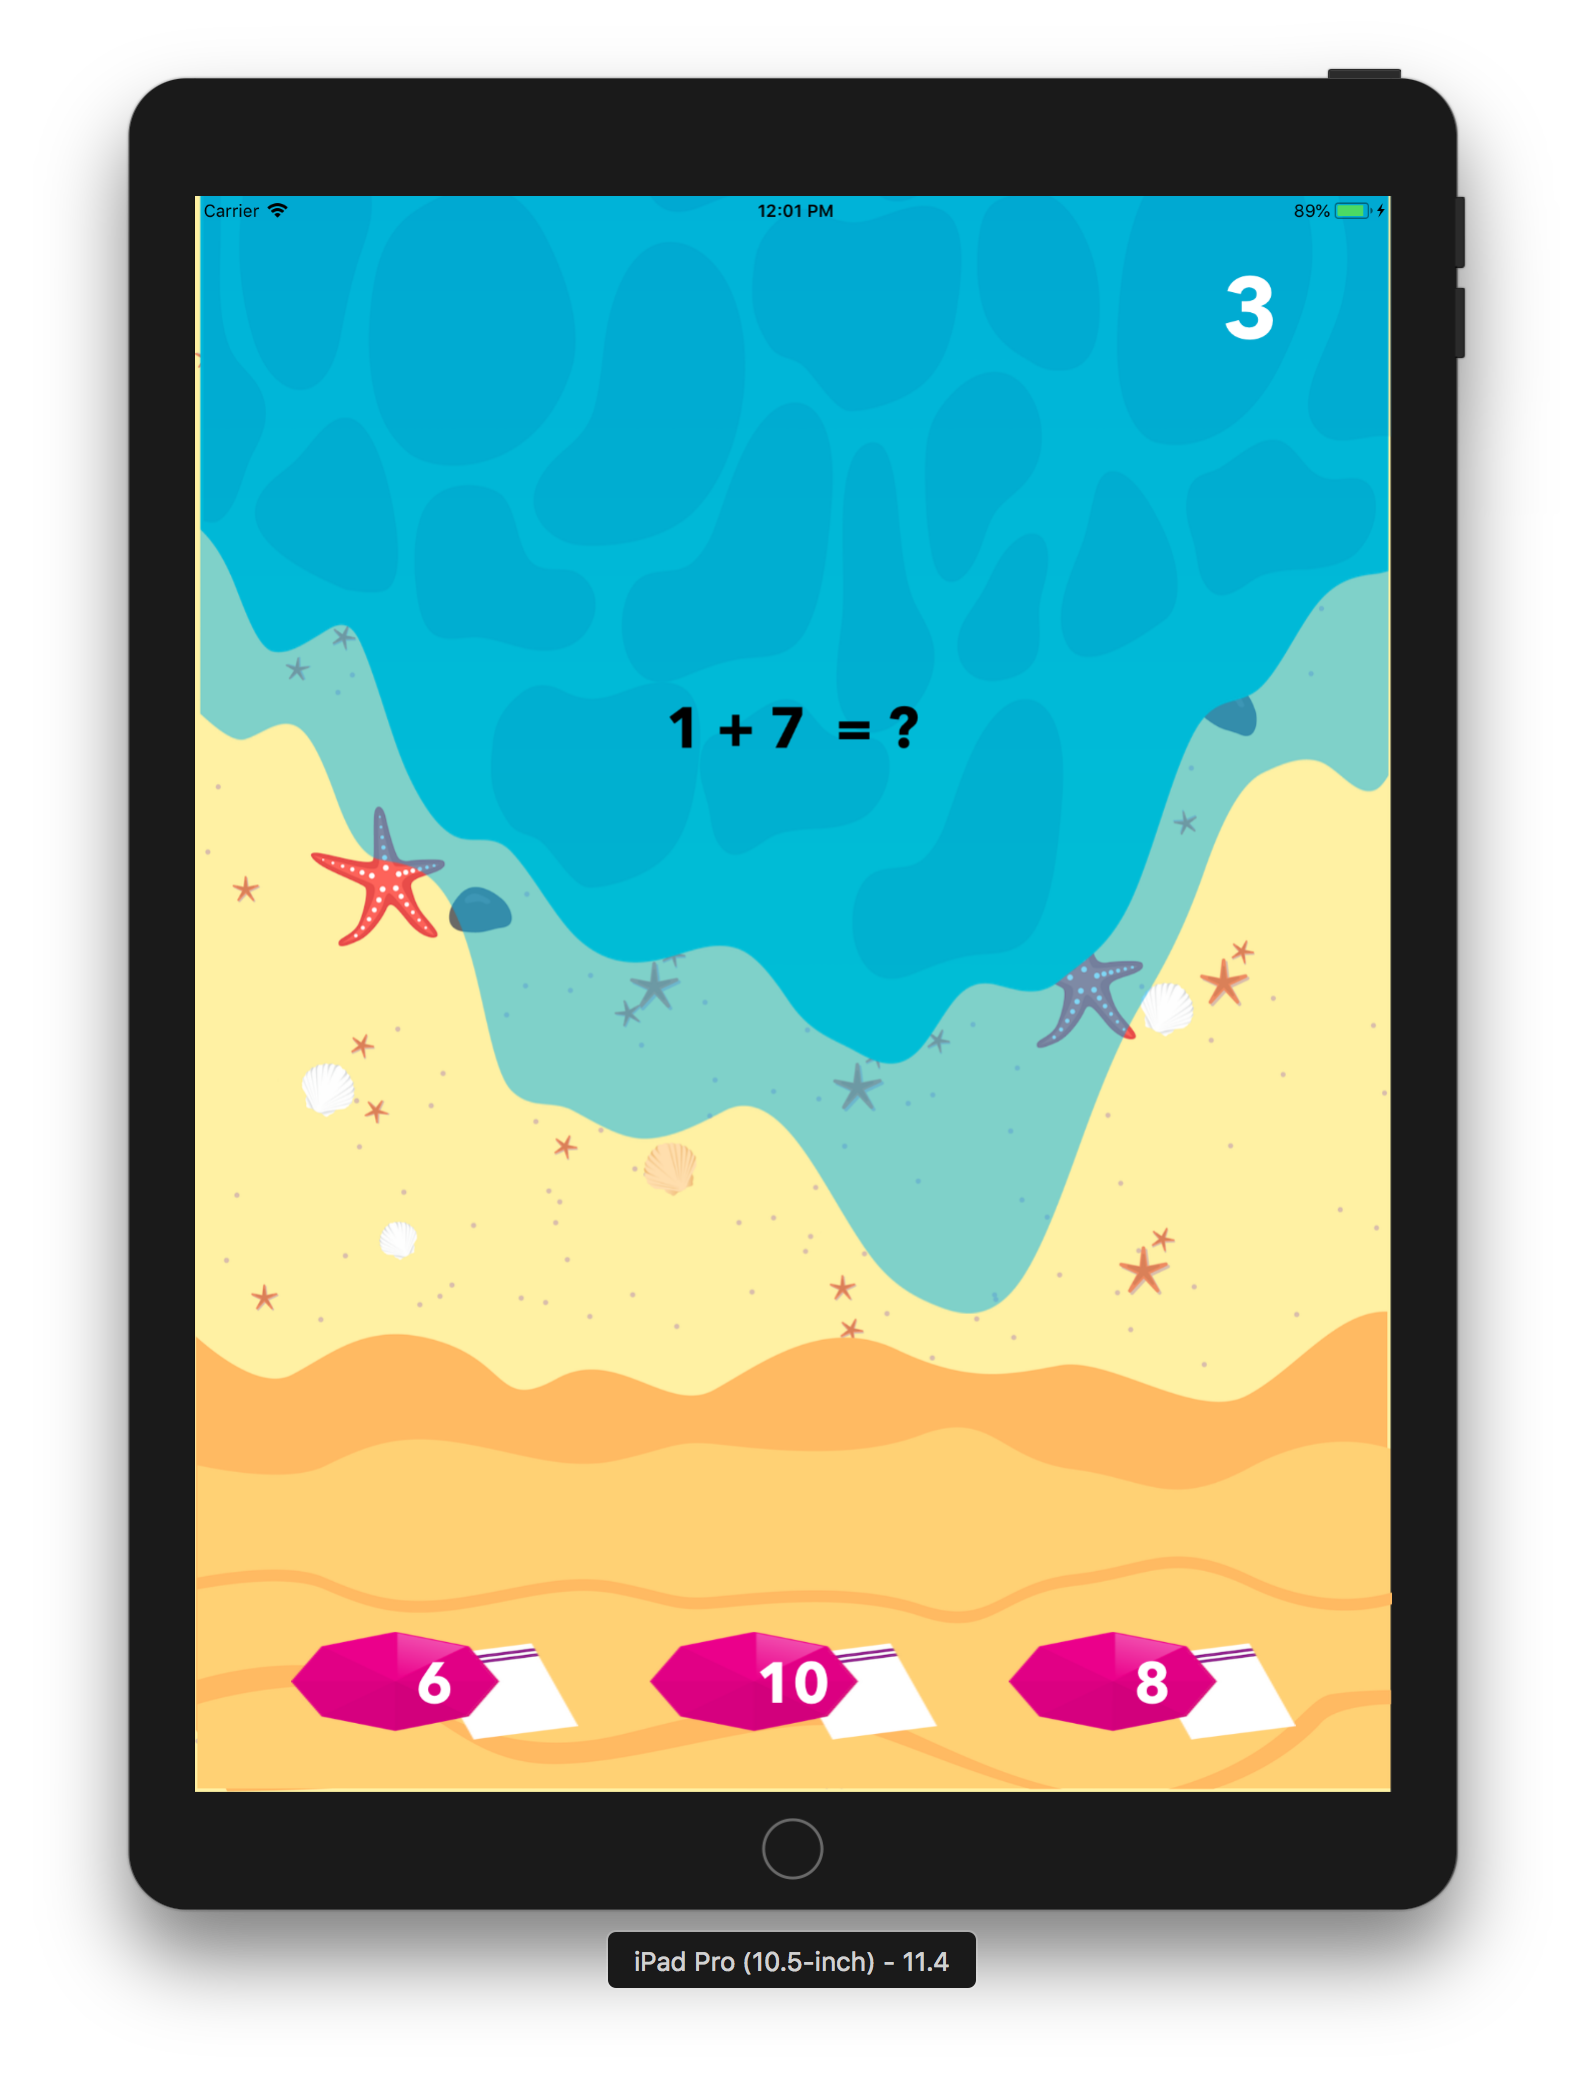
\includegraphics[width=0.5\textwidth]{images/mathPianoGame.png}
  }
	\caption{Das Mathe Piano Spiel}
	\label{Das Mathe Piano Spiel}
\end{figure}
Um das Mathepianospiel so Zielgruppen freundlich wie möglich zu gestalten, wurden verschiedene Grafiken entwickelt, welche ein typisches Strandszenario abbilden. Bei der Farbwahl wurden helle freundliche Farbtöne gewählt. Inhalt des Spiels ist eine Welle, in welcher eine Matheaufgabe abgebildet ist. Der Spieler muss die richtige Antwort auf die Matheaufgabe auswählen, bevor die Welle zu nahe kommt und die Badesachen weg spült.



\section{Fazit}
Teachify war ein herausforderendes Projekt für das 6. Semester. Dies stellte das ganze Team immer wieder vor anspruchsvolle Aufgaben. Der Umgang mit Git (\href{https://github.com/cpfeiffer3008/Teachify}{Teachify Projekt Link}) brachte zugleich viele Vorteile aber auch Herausforderungen.\\
Durch die unterschiedlichen Herangehensweisen (Design vs. Funktion) und den damit weitgehend einhergehenden Verzicht auf einen Prototypen lenkte das Projekt gegen Ende des Projektzeitraums auf einen ``Big-Bang`` Ansatz.
Positiv zu erwähnen war das Zusammenwachsen des Teams und die Zusammenarbeit untereinander. So hatten die meisten Teams eine Domäne in die sie sich eingearbeitet hatten und mussten bei der Überschneidung ihrer Gebiete zusammenarbeiten.

\section{Umsetzung des Schülerhauptmenüs \& Loginmenü}